\section{main.cpp File Reference}
\label{main_8cpp}\index{main.cpp@{main.cpp}}
{\tt \#include \char`\"{}../../LASS/src/lib.h\char`\"{}}\par
{\tt \#include $<$cstdlib$>$}\par
{\tt \#include $<$cmath$>$}\par
{\tt \#include $<$ctime$>$}\par
{\tt \#include $<$string$>$}\par
{\tt \#include $<$iostream$>$}\par
{\tt \#include \char`\"{}data\-In.h\char`\"{}}\par
{\tt \#include \char`\"{}top.h\char`\"{}}\par
{\tt \#include \char`\"{}utility.h\char`\"{}}\par
{\tt \#include \char`\"{}random.h\char`\"{}}\par
{\tt \#include \char`\"{}piece.h\char`\"{}}\par
{\tt \#include \char`\"{}lexyacc/eventparser.h\char`\"{}}\par


Include dependency graph for main.cpp:\begin{figure}[H]
\begin{center}
\leavevmode
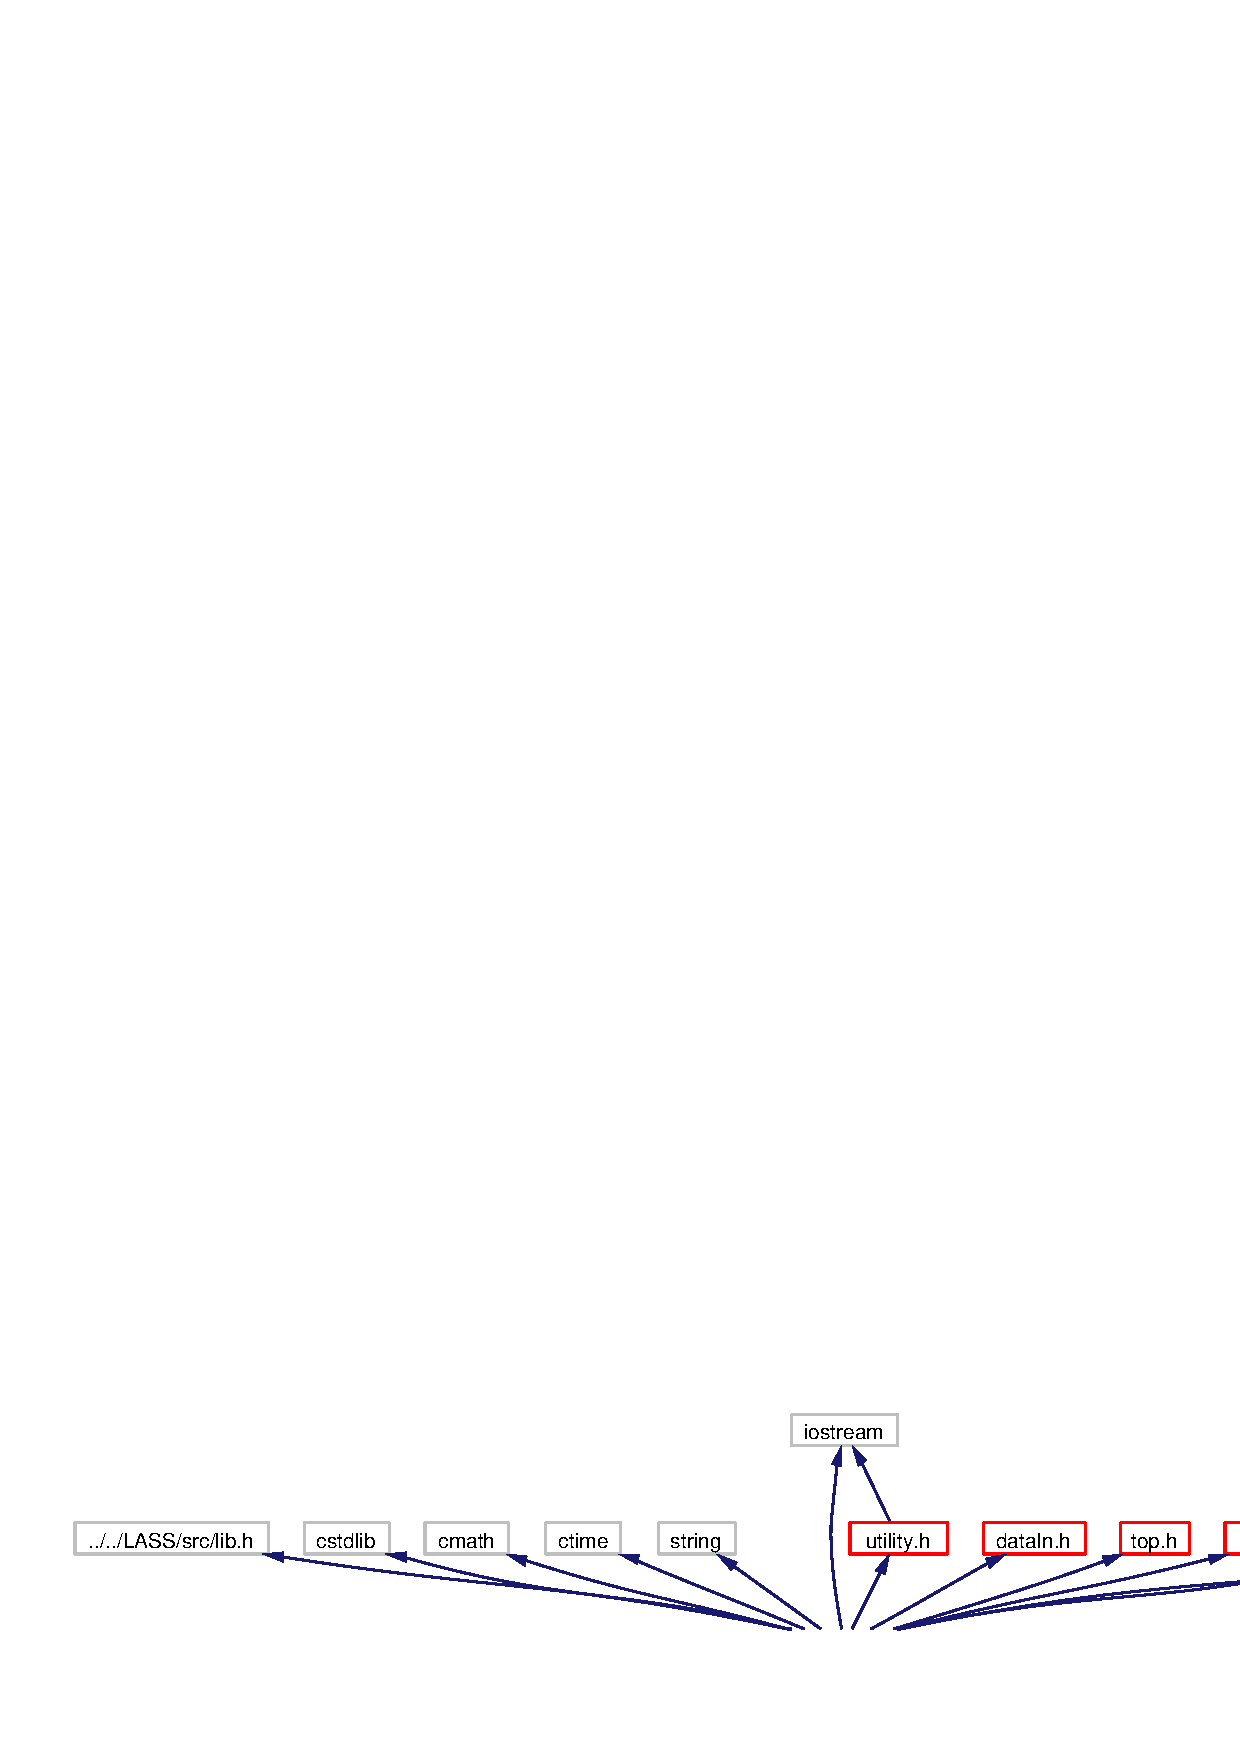
\includegraphics[width=418pt]{main_8cpp__incl}
\end{center}
\end{figure}
\subsection*{Functions}
\begin{CompactItemize}
\item 
int {\bf main} (int argc, char $\ast$$\ast$argv)
\end{CompactItemize}
\subsection*{Variables}
\begin{CompactItemize}
\item 
ofstream $\ast$ {\bf output\-File}
\item 
Envelope\-Library {\bf envlib\_\-cmod}
\item 
Score {\bf score}
\item 
vector$<$ Reverb $\ast$ $>$ {\bf reverb\-Obj\-List}
\item 
int {\bf num\-Chan}
\item 
char $\ast$ {\bf name\-Flag}
\item 
char $\ast$ {\bf file\-Name}
\item 
int {\bf sever}
\item 
{\bf CMODPiece} {\bf Piece}
\end{CompactItemize}


\subsection{Function Documentation}
\index{main.cpp@{main.cpp}!main@{main}}
\index{main@{main}!main.cpp@{main.cpp}}
\subsubsection{\setlength{\rightskip}{0pt plus 5cm}int main (int {\em argc}, char $\ast$$\ast$ {\em argv})}\label{main_8cpp_a9}


This \begin{Desc}
\item[Parameters:]
\begin{description}
\item[{\em argc}]Count of arguments passed by shell/command line \item[{\em argv}]Array of arguments set by shell/command line, as strings (char $\ast$ 's) \end{description}
\end{Desc}
\begin{Desc}
\item[Return values:]
\begin{description}
\item[{\em 0}]On success \end{description}
\end{Desc}


Definition at line 79 of file main.cpp.

References Event\-Factory::Build(), envlib\_\-cmod, CMODPiece::length, CMODPiece::num\-Channels, output\-File, Piece, CMODPiece::Print(), CMODPiece::sample\-Rate, CMODPiece::sample\-Size, score, CMODPiece::score\-Flag, CMODPiece::title, and CMODPiece::top\-File.

Here is the call graph for this function:\begin{figure}[H]
\begin{center}
\leavevmode
\includegraphics[width=357pt]{main_8cpp_a9_cgraph}
\end{center}
\end{figure}


\subsection{Variable Documentation}
\index{main.cpp@{main.cpp}!envlib_cmod@{envlib\_\-cmod}}
\index{envlib_cmod@{envlib\_\-cmod}!main.cpp@{main.cpp}}
\subsubsection{\setlength{\rightskip}{0pt plus 5cm}Envelope\-Library {\bf envlib\_\-cmod}}\label{main_8cpp_a1}




Definition at line 61 of file main.cpp.

Referenced by File\-Value::Evaluate(), and main().\index{main.cpp@{main.cpp}!fileName@{fileName}}
\index{fileName@{fileName}!main.cpp@{main.cpp}}
\subsubsection{\setlength{\rightskip}{0pt plus 5cm}char $\ast$ {\bf file\-Name}}\label{main_8cpp_a6}




Definition at line 66 of file main.cpp.

Referenced by Data\-In::Data\-In(), Data\-In::open\-File(), and Data\-In::Remember\-File\-Loc().\index{main.cpp@{main.cpp}!nameFlag@{nameFlag}}
\index{nameFlag@{nameFlag}!main.cpp@{main.cpp}}
\subsubsection{\setlength{\rightskip}{0pt plus 5cm}char$\ast$ {\bf name\-Flag}}\label{main_8cpp_a5}




Definition at line 66 of file main.cpp.\index{main.cpp@{main.cpp}!numChan@{numChan}}
\index{numChan@{numChan}!main.cpp@{main.cpp}}
\subsubsection{\setlength{\rightskip}{0pt plus 5cm}int {\bf num\-Chan}}\label{main_8cpp_a4}




Definition at line 65 of file main.cpp.\index{main.cpp@{main.cpp}!outputFile@{outputFile}}
\index{outputFile@{outputFile}!main.cpp@{main.cpp}}
\subsubsection{\setlength{\rightskip}{0pt plus 5cm}ofstream$\ast$ {\bf output\-File}}\label{main_8cpp_a0}




Definition at line 59 of file main.cpp.\index{main.cpp@{main.cpp}!Piece@{Piece}}
\index{Piece@{Piece}!main.cpp@{main.cpp}}
\subsubsection{\setlength{\rightskip}{0pt plus 5cm}{\bf CMODPiece} {\bf Piece}}\label{main_8cpp_a8}




Definition at line 70 of file main.cpp.

Referenced by Event\-Factory::Build(), Event\-Factory::Event\-Factory(), main(), and Event\-Factory::parse().\index{main.cpp@{main.cpp}!reverbObjList@{reverbObjList}}
\index{reverbObjList@{reverbObjList}!main.cpp@{main.cpp}}
\subsubsection{\setlength{\rightskip}{0pt plus 5cm}vector$<$Reverb $\ast$$>$ {\bf reverb\-Obj\-List}}\label{main_8cpp_a3}




Definition at line 64 of file main.cpp.\index{main.cpp@{main.cpp}!score@{score}}
\index{score@{score}!main.cpp@{main.cpp}}
\subsubsection{\setlength{\rightskip}{0pt plus 5cm}Score {\bf score}}\label{main_8cpp_a2}




Definition at line 62 of file main.cpp.\index{main.cpp@{main.cpp}!sever@{sever}}
\index{sever@{sever}!main.cpp@{main.cpp}}
\subsubsection{\setlength{\rightskip}{0pt plus 5cm}int {\bf sever}}\label{main_8cpp_a7}




Definition at line 68 of file main.cpp.

Referenced by Patter::Adjust(), Event::Build\-Sub\-Events(), Patter::Chooser(), Patter::Delivery(), Patter::Distort(), Event::Duration\-Methods(), Sieve::Elements(), File\-Value::Evaluate(), Patter::Expand(), Event::New\-Attack\-Methods(), Event::New\-Duration\-Methods(), Event::New\-Num\-Objs(), Event::Num\-Objs(), Bottom::Num\-Part(), Patter::Nursery(), Event::Points\-Probs(), Bottom::Rules(), Bottom::Spatialization(), Bottom::Spectrum(), Event::Sweep3(), Patter::Symmetries(), Test\-Library(), Event::Test\-Name\-Type(), Bottom::Three\-Step(), and Sieve::Weights().